\part*{Les Boss ou défis majeurs}
\markboth{}{}
\addcontentsline{toc}{part}{Les Boss ou défis majeurs}
\setcounter{tocdepth}{1}
\setcounter{chapter}{0}

\begin{figure}[H]
    \center
    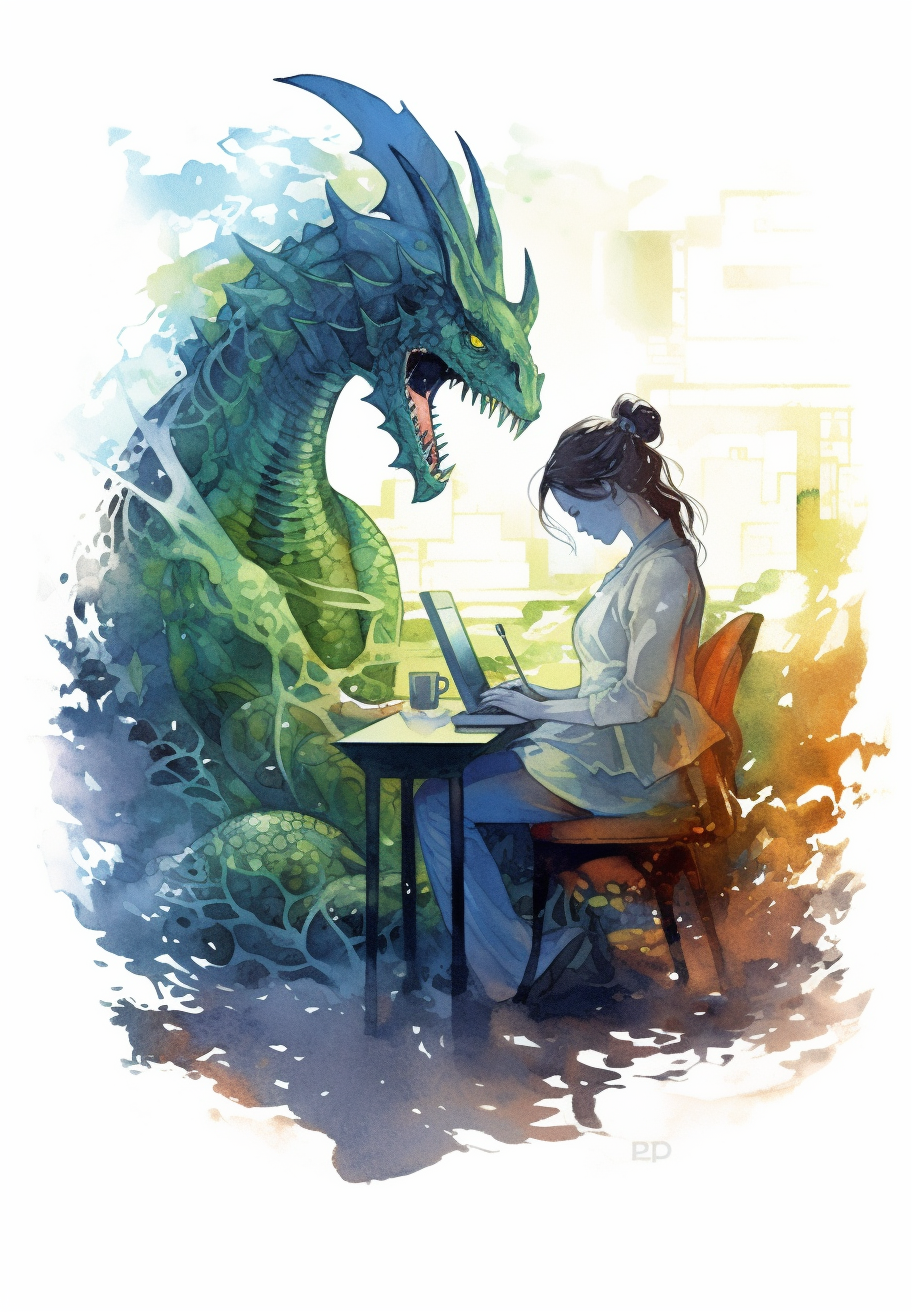
\includegraphics[keepaspectratio, width=\textwidth, height=\textheight]{images/599be801-3f3e-497a-b8d3-9b588259a13f.png}
\end{figure}

Comme dans toute quête, le parcours du·de la développeur·euse est parsemé de défis majeurs, ces "boss" qu'il faut affronter et surmonter pour progresser. Ces défis ne sont pas seulement des obstacles techniques, ils sont aussi psychologiques et sociaux, car ils touchent à nos croyances sur nous-mêmes, à notre place dans le monde du développement, et à notre capacité à nous adapter et à évoluer.

Pour un·e jeune développeur·euse, ces défis peuvent paraître intimidants, voire insurmontables. Pourtant, ils sont une partie essentielle de notre quête. En les affrontant, nous acquérons de l'expérience, nous affinons nos compétences et nous découvrons des facettes de nous-mêmes que nous ignorions.

Dans cette section, nous allons explorer trois des boss les plus courants que vous rencontrerez sur votre parcours de développeur·euse : le syndrome de l'imposteur, la complexité et le burnout. Nous allons définir ce que sont ces défis, pourquoi ils sont si redoutables, et comment les surmonter. Comme toujours, notre objectif n'est pas seulement de vous aider à survivre à ces défis, mais aussi à en tirer des leçons précieuses pour devenir un·e meilleur·e développeur·euse.

% Le Dragon du Syndrome de l'Imposteur
\chapter{Le Dragon du Syndrome de l'Imposteur}
Comment gérer le syndrome de l'imposteur.

\section{Définition et manifestations du syndrome de l'imposteur}

Le syndrome de l'imposteur est un complexe psychologique qui affecte de nombreuses personnes, en particulier dans le domaine du développement. Il se manifeste par une peur persistante d'être exposé·e comme un·e "imposteur·e", malgré des preuves évidentes de compétence et d'aptitude.

Pour le·la développeur·euse qui est confronté·e à ce dragon, cela peut signifier vivre dans la peur constante que ses collègues, ses supérieur·e·s ou même les autres membres de la communauté du développement découvrent qu'il·elle n'est pas à la hauteur, qu'il·elle n'est pas aussi compétent·e ou talentueux·euse qu'ils·elles le pensent. Cette peur peut être paralysante, et peut empêcher le·la développeur·euse d'exploiter pleinement ses talents, de prendre des risques ou d'accepter de nouvelles opportunités.

Il est important de noter que le syndrome de l'imposteur n'est pas lié à un manque réel de compétence. Au contraire, il affecte souvent les personnes les plus compétentes et les plus talentueuses, celles qui ont déjà fait leurs preuves et ont prouvé leur valeur. C'est une distorsion de la perception de soi, une forme de pensée erronée qui peut être difficile à surmonter.

\section{Pourquoi le syndrome de l'imposteur est un défi pour les développeur·euse·s}

Les développeur·euse·s sont particulièrement susceptibles d'être affecté·e·s par le syndrome de l'imposteur pour plusieurs raisons.

Premièrement, le développement est un domaine extrêmement vaste et complexe. Il est presque impossible pour une seule personne de maîtriser toutes les technologies, tous les langages de programmation, toutes les méthodologies et tous les outils qui existent. Il est donc facile de se sentir dépassé·e et de douter de ses compétences.

Deuxièmement, le développement est un domaine en constante évolution. Les technologies changent rapidement, de nouvelles méthodes sont constamment introduites, et il est essentiel de rester à jour pour rester pertinent·e. Cela peut créer une pression constante pour apprendre et s'adapter, ce qui peut à son tour alimenter le sentiment d'imposture.

Troisièmement, le développement est souvent un travail isolé. Bien que la collaboration soit une partie importante du travail, de nombreux·euses développeur·euse·s passent de longues heures seul·e·s devant leur ordinateur. Cela peut rendre difficile l'établissement de comparaisons justes avec les compétences et les réalisations des autres, et peut amplifier les sentiments d'imposture.

\section{Stratégies pour combattre le syndrome de l'imposteur}

Heureusement, même si le syndrome de l'imposteur est un adversaire redoutable, il existe des stratégies efficaces pour le combattre.

\begin{itemize}
    \item \textbf{Reconnaître et nommer le syndrome de l'imposteur :} La première étape pour vaincre ce dragon est de le reconnaître pour ce qu'il est : un complexe psychologique basé sur une perception erronée de soi. Il est normal de douter de soi de temps en temps, mais quand ces doutes deviennent envahissants et paralysants, il est important de les identifier comme tels.
    \item \textbf{Se rappeler de ses réalisations :} Une autre stratégie efficace consiste à se rappeler régulièrement de ses réalisations et de ses succès. Il peut être utile de tenir un journal des succès, où l'on note les projets que l'on a menés à bien, les problèmes que l'on a résolus, les compliments que l'on a reçus, etc. Ceci peut aider à contrebalancer les pensées négatives et à renforcer l'estime de soi.
    \item \textbf{Partager ses sentiments avec d'autres :} Le syndrome de l'imposteur a tendance à prospérer dans le secret et l'isolement. En partageant vos sentiments avec des collègues de confiance, des mentors ou des ami·e·s, vous pouvez briser ce cercle vicieux. Vous serez probablement surpris·e de découvrir que beaucoup d'entre eux·elles ont eu les mêmes sentiments.
    \item \textbf{Rechercher un soutien professionnel :} Si le syndrome de l'imposteur est particulièrement envahissant et affecte votre qualité de vie ou votre performance au travail, il peut être utile de consulter un·e professionnel·le de la santé mentale. Un·e thérapeute ou un·e coach peut vous aider à comprendre et à surmonter ces sentiments.
\end{itemize}

En conclusion, le syndrome de l'imposteur est un défi majeur pour de nombreux·euses développeur·euse·s, mais il peut être surmonté. En reconnaissant ce syndrome pour ce qu'il est, en valorisant vos réalisations, en partageant vos sentiments et en recherchant un soutien, vous pouvez vaincre ce dragon et continuer à progresser dans votre parcours de développeur·euse.



% Le Golem de la Complexité
\chapter{Le Golem de la Complexité}
Comment aborder des projets complexes et les rendre gérables.

\section{Confrontation avec la complexité dans le développement}

Le monde du développement est parsemé de projets complexes. Que vous soyez un·e développeur·euse débutant·e travaillant sur votre premier projet majeur ou un·e expert·e chevronné·e abordant une nouvelle technologie ou un nouveau domaine d'application, la complexité est une réalité incontournable. La complexité peut prendre de nombreuses formes, que ce soit le nombre de composants interdépendants d'un système, l'incertitude inhérente à un projet ou la nouveauté d'une technologie ou d'un domaine. Comprendre comment appréhender et gérer la complexité est une compétence essentielle pour tout·e développeur·euse.

\section{La nature du Golem de la Complexité}

Dans le folklore juif, un golem est une créature formée à partir de matières inanimées, souvent de l'argile ou de la boue, animé par un rituel magique. Un golem peut être un serviteur utile, mais il peut aussi devenir incontrôlable et destructeur si son maître ne prend pas les précautions nécessaires. De la même manière, la complexité d'un projet peut être un outil précieux qui permet de créer des systèmes puissants et flexibles, mais elle peut aussi devenir incontrôlable et déstabilisante si elle n'est pas correctement gérée.

\section{Stratégies pour appréhender la complexité}

\subsection{Décomposition du problème}
Une des stratégies les plus efficaces pour gérer la complexité est de décomposer un problème complexe en sous-problèmes plus petits et plus gérables. Chaque sous-problème peut alors être résolu séparément, rendant la tâche globale moins intimidante.

\subsection{Abstraction}
L'abstraction est un autre outil puissant pour gérer la complexité. En regroupant les détails de mise en œuvre dans des fonctions, des classes ou des modules, vous pouvez concentrer votre attention sur un niveau plus élevé de fonctionnalité sans être submergé·e par les détails.

\subsection{Test et débogage progressifs}
Lorsque vous travaillez sur un projet complexe, il est crucial de ne pas attendre la fin pour tester votre code. En intégrant des tests et du débogage tout au long du processus de développement, vous pouvez attraper et résoudre les problèmes plus tôt, évitant ainsi une accumulation de problèmes qui pourrait rendre le débogage final presque impossible.

\subsection{Documentation}
Une bonne documentation est un élément essentiel pour gérer la complexité. Une documentation claire et complète peut aider à clarifier la structure et le fonctionnement d'un projet complexe, et peut servir de guide précieux lorsque vous (ou d'autres développeur·euse·s) devez travailler sur le projet à l'avenir.

\section{Gérer le Golem : un élément clé du développement}

Gérer la complexité est une compétence clé dans le développement. En apprenant à décomposer les problèmes, à utiliser l'abstraction, à tester et déboguer progressivement, et à documenter soigneusement votre travail, vous pouvez rendre n'importe quel projet, aussi complexe soit-il, gérable et réussi. Rappelez-vous que même le Golem le plus intimidant peut être apprivoisé avec les bonnes stratégies.

\section{Établissement de normes et de conventions de codage}

Une autre stratégie pour gérer la complexité consiste à établir des normes et des conventions de codage. Lorsque vous travaillez sur un grand projet, en particulier en équipe, il est important de vous assurer que tout le monde utilise le même style de codage. Cela permet de rendre le code plus lisible et plus compréhensible, et aide à prévenir les erreurs et les problèmes qui peuvent survenir lorsque différentes parties du code sont écrites de manière différente. Il peut être utile d'utiliser un outil d'analyse de code statique ou un linter pour vérifier automatiquement la conformité aux normes de codage.

\section{Utilisation de modèles de conception}

Les modèles de conception sont des solutions éprouvées à des problèmes de conception communs. Ils peuvent être extrêmement utiles pour gérer la complexité, car ils fournissent des structures prédéfinies qui peuvent aider à organiser le code et à rendre la structure du projet plus claire et plus compréhensible. Les modèles de conception peuvent également aider à éviter certains problèmes courants en fournissant des approches standardisées pour résoudre des problèmes communs.

\section{Investissement dans l'apprentissage continu}

La technologie évolue rapidement, et ce qui peut sembler complexe et déroutant aujourd'hui peut devenir plus facile à comprendre à mesure que vous continuez à apprendre et à vous développer en tant que développeur·euse. Investir du temps dans l'apprentissage continu, que ce soit par la lecture de livres, la participation à des cours en ligne, l'assistance à des conférences, ou simplement la pratique et l'expérimentation, peut vous aider à développer les compétences et les connaissances nécessaires pour gérer la complexité.

\section{La complexité n'est pas toujours une mauvaise chose}

Il est important de se rappeler que la complexité n'est pas toujours une mauvaise chose. En fait, dans de nombreux cas, la complexité est une conséquence nécessaire de la création de systèmes puissants et flexibles. La clé est de savoir comment gérer cette complexité de manière efficace. En décomposant les problèmes, en utilisant l'abstraction, en testant et en déboguant progressivement, en documentant soigneusement votre travail, en respectant les normes et conventions de codage, en utilisant les modèles de conception, et en investissant dans l'apprentissage continu, vous pouvez prendre le contrôle du Golem de la Complexité et faire de lui un allié plutôt qu'un adversaire.

\section{Conclusion}

Tout comme un Golem peut être un serviteur puissant si on sait le contrôler, la complexité peut être une force si elle est correctement gérée. En adoptant une approche méthodique et stratégique de la complexité, vous pouvez transformer ce qui pourrait autrement être un obstacle insurmontable en une partie intégrante du processus de création de systèmes de logiciels puissants et efficaces.



% Le Titan du Burnout
\chapter{Le Titan du Burnout}
Comment prévenir et gérer le burnout en développement

\section{Introduction}

Dans le royaume du développement logiciel, il existe un adversaire qui peut s'avérer plus redoutable que tout autre : le Titan du Burnout. Comme le suggère son nom, cet adversaire ne vient pas sous la forme d'un bug de code particulier ou d'un problème de déploiement complexe, mais plutôt comme une menace pour votre santé mentale et votre bien-être. Le burnout est un état d'épuisement émotionnel, mental et physique causé par un stress prolongé ou excessif. Il est particulièrement prévalent dans les professions à forte charge cognitive et à haute pression, comme le développement de logiciels. En tant que développeur·se, vous êtes susceptible de rencontrer le Titan du Burnout à un moment ou à un autre de votre carrière, il est donc crucial de savoir comment prévenir et gérer ce défi redoutable.

\section{Reconnaître les signes du burnout}

Le burnout ne survient pas du jour au lendemain. Il se développe progressivement, souvent à partir d'un stress chronique non géré. Apprendre à reconnaître les signes précoces du burnout peut vous aider à prendre des mesures pour prévenir son apparition. Voici quelques signes courants de burnout à surveiller :

\begin{itemize}
    \item Épuisement émotionnel et physique : vous vous sentez vidé·e et incapable de faire face aux demandes de votre travail.
    \item Cynisme et déconnexion : vous pouvez vous sentir distancié·e de votre travail, devenir cynique ou négatif·ve à son égard, ou avoir du mal à trouver de la satisfaction dans ce que vous faites.
    \item Sentiments d'inefficacité : vous pouvez avoir l'impression de ne pas accomplir grand-chose, ou de ne pas être à la hauteur de vos propres attentes ou de celles des autres.
    \item Problèmes de sommeil : le stress chronique peut perturber votre sommeil, ce qui peut aggraver encore les symptômes du burnout.
    \item Problèmes de santé : le stress chronique peut également avoir un impact sur votre santé physique, en contribuant à des problèmes tels que des maux de tête, des douleurs musculaires, des problèmes digestifs et une pression artérielle élevée.
\end{itemize}

\section{Stratégies pour prévenir le burnout}

La prévention est la meilleure défense contre le Titan du Burnout. Voici quelques stratégies que vous pouvez utiliser pour maintenir votre équilibre et prévenir le burnout :

\subsection{Établir des limites}

Une des clés pour prévenir le burnout est de définir et de respecter des limites claires entre votre travail et votre vie personnelle. Cela peut impliquer de définir des heures de travail spécifiques, de prendre des pauses régulières et de vous assurer que vous avez du temps pour vous détendre et vous déconnecter du travail. Il peut être particulièrement important d'établir ces limites si vous travaillez à domicile ou si vous avez des heures de travail flexibles.

\subsection{Prendre soin de votre santé physique}

L'exercice régulier, une alimentation saine et un sommeil suffisant sont tous essentiels pour maintenir votre bien-être physique et mental. Ils peuvent également vous aider à mieux gérer le stress et à prévenir le burnout. Essayez de faire de ces activités une priorité, même lorsque vous êtes occupé·e.

\subsection{Développer des stratégies de gestion du stress}

La gestion du stress est une compétence essentielle pour tout développeur·se. Cela peut impliquer des techniques de relaxation, comme la méditation ou la respiration profonde, ou des activités qui vous aident à vous détendre et à vous déstresser, comme la lecture, la musique ou l'art.

\subsection{Chercher un soutien}

Il peut être très utile de parler de vos sentiments et de vos préoccupations à quelqu'un en qui vous avez confiance, que ce soit un ami·e, un membre de votre famille, un·e collègue ou un·e conseiller·ère professionnel·le. Le soutien social peut être un excellent tampon contre le stress et le burnout.

\subsection{Faire preuve de compassion envers vous-même}

Enfin, il est important de se rappeler que personne n'est parfait·e, et que tout le monde fait face à des défis et à des difficultés. Faire preuve de compassion envers vous-même, en reconnaissant vos efforts et en vous donnant la permission de faire des erreurs ou de prendre du temps pour vous-même, peut être un outil puissant pour prévenir le burnout.

\section{Gérer le burnout}

Si vous êtes déjà en proie au Titan du Burnout, il est important de prendre des mesures pour gérer la situation. Voici quelques stratégies qui peuvent vous aider :

\subsection{Reconnaître et accepter la situation}

La première étape pour gérer le burnout est de reconnaître et d'accepter qu'il se produit. Il est normal de traverser des périodes de stress et d'épuisement, et il est important de ne pas vous juger ou vous critiquer pour ressentir ces sentiments.

\subsection{Chercher du soutien}

Si vous êtes en situation de burnout, il est essentiel de chercher du soutien. Cela peut impliquer de parler de vos sentiments à un·e professionnel·le de la santé mentale, comme un·e psychologue ou un·e conseiller·ère. Si vous vous sentez à l'aise de le faire, vous pourriez également vouloir en parler à votre manager ou à vos collègues pour voir s'il y a des aménagements qui peuvent être faits pour alléger votre charge de travail.

\subsection{Faire des changements dans votre vie professionnelle}

Dans certains cas, il peut être nécessaire de faire des changements plus importants dans votre vie professionnelle pour gérer le burnout. Cela pourrait impliquer de chercher des moyens de réduire votre charge de travail, de réévaluer vos priorités ou de changer d'environnement de travail.

\subsection{Prendre soin de vous-même}

Prendre soin de vous-même est essentiel pour la récupération du burnout. Cela peut impliquer de prendre du temps pour vous reposer et vous relaxer, de faire de l'exercice, de manger sainement et de dormir suffisamment.

\section{Conclusion}

Le Titan du Burnout est un adversaire redoutable, mais avec les bonnes stratégies et le soutien, vous pouvez le vaincre. En apprenant à reconnaître les signes du burnout, en mettant en place des stratégies de prévention et en prenant des mesures pour gérer le burnout lorsqu'il survient, vous pouvez maintenir votre bien-être mental et physique et continuer à prospérer dans votre carrière en développement.

